\documentclass[a4paper,12pt]{article}   % papír A4, písmo 12 bodu
\usepackage[utf8x]{inputenc}            %kodovaní UTF-8
\usepackage{ucs}                        %kodovani unicode
\usepackage[czech]{babel}               %podpora cestiny
\usepackage[T1]{fontenc}                %pouzij variantu pisma T1 (hacky, carky)
\usepackage[left=2.5cm,right=1.5cm,top=2.5cm,bottom=2.5cm]{geometry} %okraje stranky
\usepackage{amsmath,amsfonts,amssymb}   %podpora matematiky
\usepackage{gensymb,marvosym}           %symboly celsius (\celsius) apod.
%\usepackage{mathptmx}                   %font Times New Roman s~podporou matematiky
\usepackage{times}                      %font Times New Roman (matematika pismem Computer Modern) 
\usepackage{parskip}                    %mezera mezi odstavci
%\usepackage[document]{ragged2e}         %text zarovany vlevo
\usepackage[none]{hyphenat} \sloppy     %slova nedelit a~nepretekat
\usepackage{titlesec}
\setcounter{secnumdepth}{4}
\clubpenalty 10000                      %kontrolovat sirotky
\widowpenalty 10000                     %kontrolovat vdovy
\usepackage{setspace} \onehalfspacing   %podpora pro zmenu radkovani + radkovani 1,5
\usepackage{enumerate}                  %podpora pro zmenu cislovani
\usepackage{fancyhdr}                   %vlastni zahlavi a~zapati
\usepackage{graphicx}                   %podpora grafiky
\graphicspath{{materialy/}}                   %vychozi adresar s~obrazky
\usepackage{caption}                    %popisky
\usepackage{subcaption}                 %podpopisky
\usepackage{siunitx}
\usepackage{MnSymbol,wasysym}
\usepackage[shortlabels]{enumitem}
\usepackage{amsmath}
\usepackage{lastpage}                   %zjištění poslední stránky \pageref{LastPage}
\usepackage{float}                      
\usepackage{url}
\usepackage[unicode]{hyperref}          %klikaci odkazy v textu
\usepackage{mhchem}
\usepackage{multirow}

\usepackage{halloweenmath}


\titleclass{\subsubsubsection}{straight}[\subsection]
\newcounter{subsubsubsection}[subsubsection]
\renewcommand\thesubsubsubsection{\thesubsubsection.\arabic{subsubsubsection}}
\renewcommand\theparagraph{\thesubsubsubsection.\arabic{paragraph}} % optional; useful if paragraphs are to be numbered


%------------------------ čtvrtá a pátá úroveň nadpisu ---------------------------

\titleformat{\subsubsubsection}
  {\normalfont\normalsize\bfseries}{\thesubsubsubsection}{1em}{}
\titlespacing*{\subsubsubsection}
{0pt}{3.25ex plus 1ex minus .2ex}{1.5ex plus .2ex}

\makeatletter

\renewcommand\paragraph{\@startsection{paragraph}{5}{\z@}%
  {3.25ex \@plus1ex \@minus.2ex}%
  {-1em}%
  {\normalfont\normalsize\bfseries}}
\renewcommand\subparagraph{\@startsection{subparagraph}{6}{\parindent}%
  {3.25ex \@plus1ex \@minus .2ex}%
  {-1em}%
  {\normalfont\normalsize\bfseries}}
\def\toclevel@subsubsubsection{4}
\def\toclevel@paragraph{5}
\def\toclevel@paragraph{6}
\def\l@subsubsubsection{\@dottedtocline{4}{7em}{4em}}
\def\l@paragraph{\@dottedtocline{5}{10em}{5em}}
\def\l@subparagraph{\@dottedtocline{6}{14em}{6em}}
\makeatother

\setcounter{secnumdepth}{4}
\setcounter{tocdepth}{4}


\setlist[enumerate]{itemsep=0mm}
%_____________________________|___________________________|_____________________________%
%                             |                           |                             %
%-----------------------------| ZDE VYPLNIT UDAJE O PRACI |-----------------------------%
%_____________________________|___________________________|_____________________________%
%                             

\newcommand{\nazev}{MĚŘENÍ MALÝCH PROUDŮ}                                                        %
\newcommand{\jmeno}{Jakub Dvořák}                                                     %
\newcommand{\datum}{18.10.2020}                                                              %
%---------------------------------------------------------------------------------------%


%-----------------------------| POUŽITÁ MAKRA |-----------------------------%

%\newcommand{\zkratka}{ve výsledku se mi napíše tenhle text}
%\newcommand{}{}
%\newcommand{}{}
%\newcommand{}{}
\newcommand{\tsub}[1]{$_\textrm{#1}$}
\newcommand{\texp}[1]{$^\textrm{#1}$}
\newcommand{\tmu}{$\mu$}

%_______________________________________________________________________________________%
%_______________________________________________________________________________________%


%----------------------------------- KONEC PREAMBULE -----------------------------------%






%-------------------------------------- DOKUMENT --------------------------------------%
%______________________________________________________________________________________%
\begin{document} %%%%%%%%%%%%%%%%%%%%%%%%%%%%%%%%%%%%%%%%%%%%%%%%%%%%%%%%%%%%%%%%%%%%%%%

\setcounter{page}{0} %cislo strany
\pagestyle{empty} %stranku necislovat

%prostredi pro grafy a schemata \begin{graf} \begin{schema}
\newfloat{schema}{htbp}{schema}\floatname{schema}{Schéma}
\newfloat{graf}{htbp}{graf}\floatname{graf}{Graf}

\begin{titlepage}
    \begin{center}
        \vspace*{1cm}
            
        \Huge
        \textbf{\nazev}
            
        \vspace{0.5cm}
        \LARGE
            
        \vspace{1.5cm}
            
        \textbf{\jmeno}
            
        \vfill
            
        \vspace{0.8cm}
            
        \Large
            
        \datum\\
        \vspace*{.5cm}
        
\includegraphics[width=.4\textwidth]{logo-cvut-fee.png}\\
    \end{center}
\end{titlepage}

% --- definice zapati a~cislovani ---
\newpage 
\pagestyle{fancy}                                       %vlastni zahlavi/zapati
\renewcommand{\headrulewidth}{0pt}                      %bez linky v~zahlavi
\renewcommand{\footrulewidth}{.5pt}                    %linka v~zapati - optional
\lhead{}       \chead{} \rhead{}                        %pole zahlavi (prazdna)
\lfoot{\nazev} \cfoot{} \rfoot{\thepage}   %pole zapati


%------------------------------------ VLASTNÍ TEXT ------------------------------------%



\section{Úkol měření}
\label{zadani}
\begin{enumerate}
    \item V zapojení podle obr. \ref{fig:schema} změřte proud germaniovou diodou v propustném směru v oblasti malých napětí (20 až 100 mV) v pěti bodech charakteristiky:\label{jedna}
    \begin{enumerate}[label=\alph*)]
        \item analogovým mikroampérmetrem,\label{analog}
        \item číslicovým mikroampérmetrem na různých rozsazích,\label{digital}
        \item pomocí převodníku proud - napětí s operačním zesilovačem, u něhož před měřením určete velikost odporu zpětnovazebního rezistoru R tak, aby převod proud - napětí byl 10\texp{-5} A/V.
    \end{enumerate}
    \item Naměřené hodnoty vyneste do společného grafu.
    \item Při měření dle \ref{jedna}\ref{analog} a \ref{jedna}\ref{digital} určete chybu metody způsobenou vnitřním odporem ampérmetru.
    \item Z naměřených hodnot určete \textbf{vnitřní odpory použitých mikroampérmetrů}.
\end{enumerate}

\section{Schéma zapojení}
\label{schema_zapojeni}
\begin{figure}[h!]
    \centering
    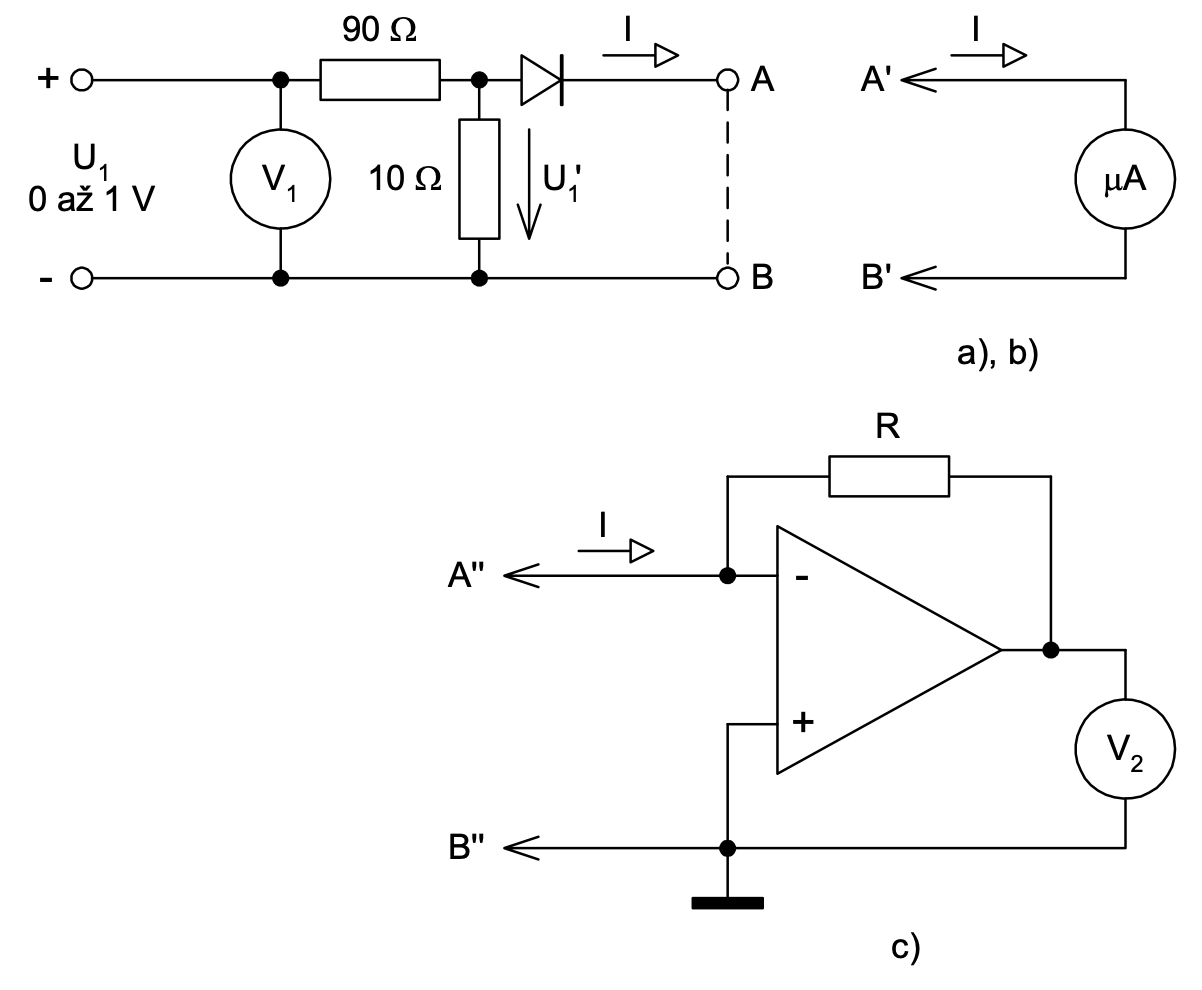
\includegraphics[width=.8\textwidth]{schema.png}
    \caption{Zapojení pro měření malých proudů \cite{navod}}
    \label{fig:schema}
\end{figure}


\section{Seznam použitých přístrojů}
\begin{itemize}
    \item V\tsub{2} - voltmetr číslicový, typ ..., přesnost ...
    \item $\mu$A\tsub{1} - mikroampérmetr magnetoelektrický, tř.přes. ..., rozsah ...
    \item $\mu$A\tsub{2} - mikroampérmetr číslicový, typ ..., přesnost ...
    \item R - přesný rezistor nebo odporová dekáda, přesnost 0,1\,\% (příp. 0,2\,\%)
    \item Př1 - přípravek s odporovým děličem a polovodičovou diodou
    \item Př2 - přípravek s operačním zesilovačem
    \item U\tsub{1} - zdroj proměnného stejnosměrného napětí s číslicově nastavitelnou hodnotou 
    \item NZ - napájecí zdroj pro OZ
\end{itemize}

\section{Teoretický úvod}
Při měření malých proudů ručními ampérmetry nastává chyba měření. Ta je dána relativně vysokým odporem bočníku ampérmetru, na kterém měříme úbytek napětí. Dle obrázku \ref{fig:schema} je vidět, že odpor diody, která není vlivem nízkého napětí zcela otevřena, je srovnatelný s odporem ampérmetru. Vinou čehož vznikne dělič napětí se srovnatelnými úbytky napětí na diodě a na ampérmetru. Tato chyba metody jde kompenzovat zvýšením rozsahu a tedy snížením odporu. Zde se ale naměřená hodnota dostane na začátek rozsahu a vzniká zde opět nejistota měření daná \textit{chybou rozsahu}. 


\section{Naměřené hodnoty}
Změřená data jsou v tabulce \ref{tab:zmereno}.

\begin{table}[h!]
    \begin{tabular}{|c|c|c|c|c|}
        \hline
        \rule{0pt}{2.5ex}
        \multirow{2}{*}{Vstupní napětí $\frac{U}{\textrm{V}}$}& Ručičkový \tmu ampérmetr$\frac{I}{\mu\textrm{A}}$ 	&GDM-8145 $\frac{I}{\mu\textrm{A}}$	&GDM-8145 $\frac{I}{\textrm{mA}}$	&IU Převodník $\frac{U}{\textrm{V}}$  \\[.7ex]
        & rozsah  150~μA & rozsah 200~μA & rozsah  2~mA & rozsah  2 V\\\hline\hline
        0,2&0,9&1,33&0,0012&-0,0155\\\hline
        0,3&1,4&2,36&0,0024&-0,0277\\\hline
        0,4&2&3,69&0,0041&-0,0448\\\hline
        0,5&2,6&5,39&0,0064&-0,0684\\\hline
        0,6&3,3&7,48&0,0095&-0,1012\\\hline
        0,7&4&10&0,0136&-0,1459\\\hline
        0,8&4,8&12,96&0,0190&-0,2062\\\hline
        0,9&5,25&16,37&0,0260&-0,2867\\\hline
        1&6,4&20,23&0,0349&-0,3926\\\hline
    
    \end{tabular}
    \caption{Změřené hodnoty}
    \label{tab:zmereno}
\end{table}

Námi změřené hodnoty mají různé předpony i jednotky. Je proto nutné je přepočítat na jednotné jednotky. Pro číslicový ampérmetr stačí hodnoty v mA vynásobit 1000, abychom dostali \tmu A. Pro spočtení napětí na výstupu operačního zesilovače platí:
\begin{equation*}
    \begin{split}
        I_{in}&=-I_{out}\\
        I_{in}&=-\frac{U_{out}}{R}\\
        I_{in}&=-\frac{U_{out}}{10\,000} \textrm{A}\\
    \end{split}
\end{equation*}
Jelikož hodnoty napětí byly měřeny ve voltech a jednotné jednotky jsou \tmu A, je potřeba změřené napětí vydělit $-0,1\,\frac{\textrm{A}}{\textrm{V}}$. Přepočtené hodnoty jsou zapsána v tabulce \ref{tab:prepocteno} a zobrazena v grafu \ref{graf:hodnoty}.


\begin{table}[h!]
    \begin{tabular}{|c|c|c|c|c|}
        \hline
        \rule{0pt}{2.5ex}
        \multirow{2}{*}{Vstupní napětí $\frac{U}{\textrm{V}}$}& Ručičkový \tmu ampérmetr$\frac{U}{\mu\textrm{A}}$ 	&GDM-8145 $\frac{U}{\mu\textrm{A}}$	&GDM-8145 $\frac{U}{\mu\textrm{A}}$	&IU Převodník $\frac{I}{\mu\textrm{A}}$  \\[.7ex]
        & rozsah  150~μA & rozsah 200~μA & rozsah  2~mA & rozsah  2 V\\\hline\hline
        0,02&0,9&1,33&1,2&1,55\\\hline
        0,03&1,4&2,36&2,4&2,77\\\hline
        0,04&2&3,69&4,1&4,48\\\hline
        0,05&2,6&5,39&6,4&6,84\\\hline
        0,06&3,3&7,48&9,5&10,12\\\hline
        0,07&4&10&13,6&14,59\\\hline
        0,08&4,8&12,96&19&20,62\\\hline
        0,09&5,25&16,37&26&28,67\\\hline
        0,1&6,4&20,23&34,9&39,26\\\hline
    \end{tabular}
    \caption{Přepočtené hodnoty}
    \label{tab:prepocteno}
\end{table}

\begin{graf}[h!]
    \centering
    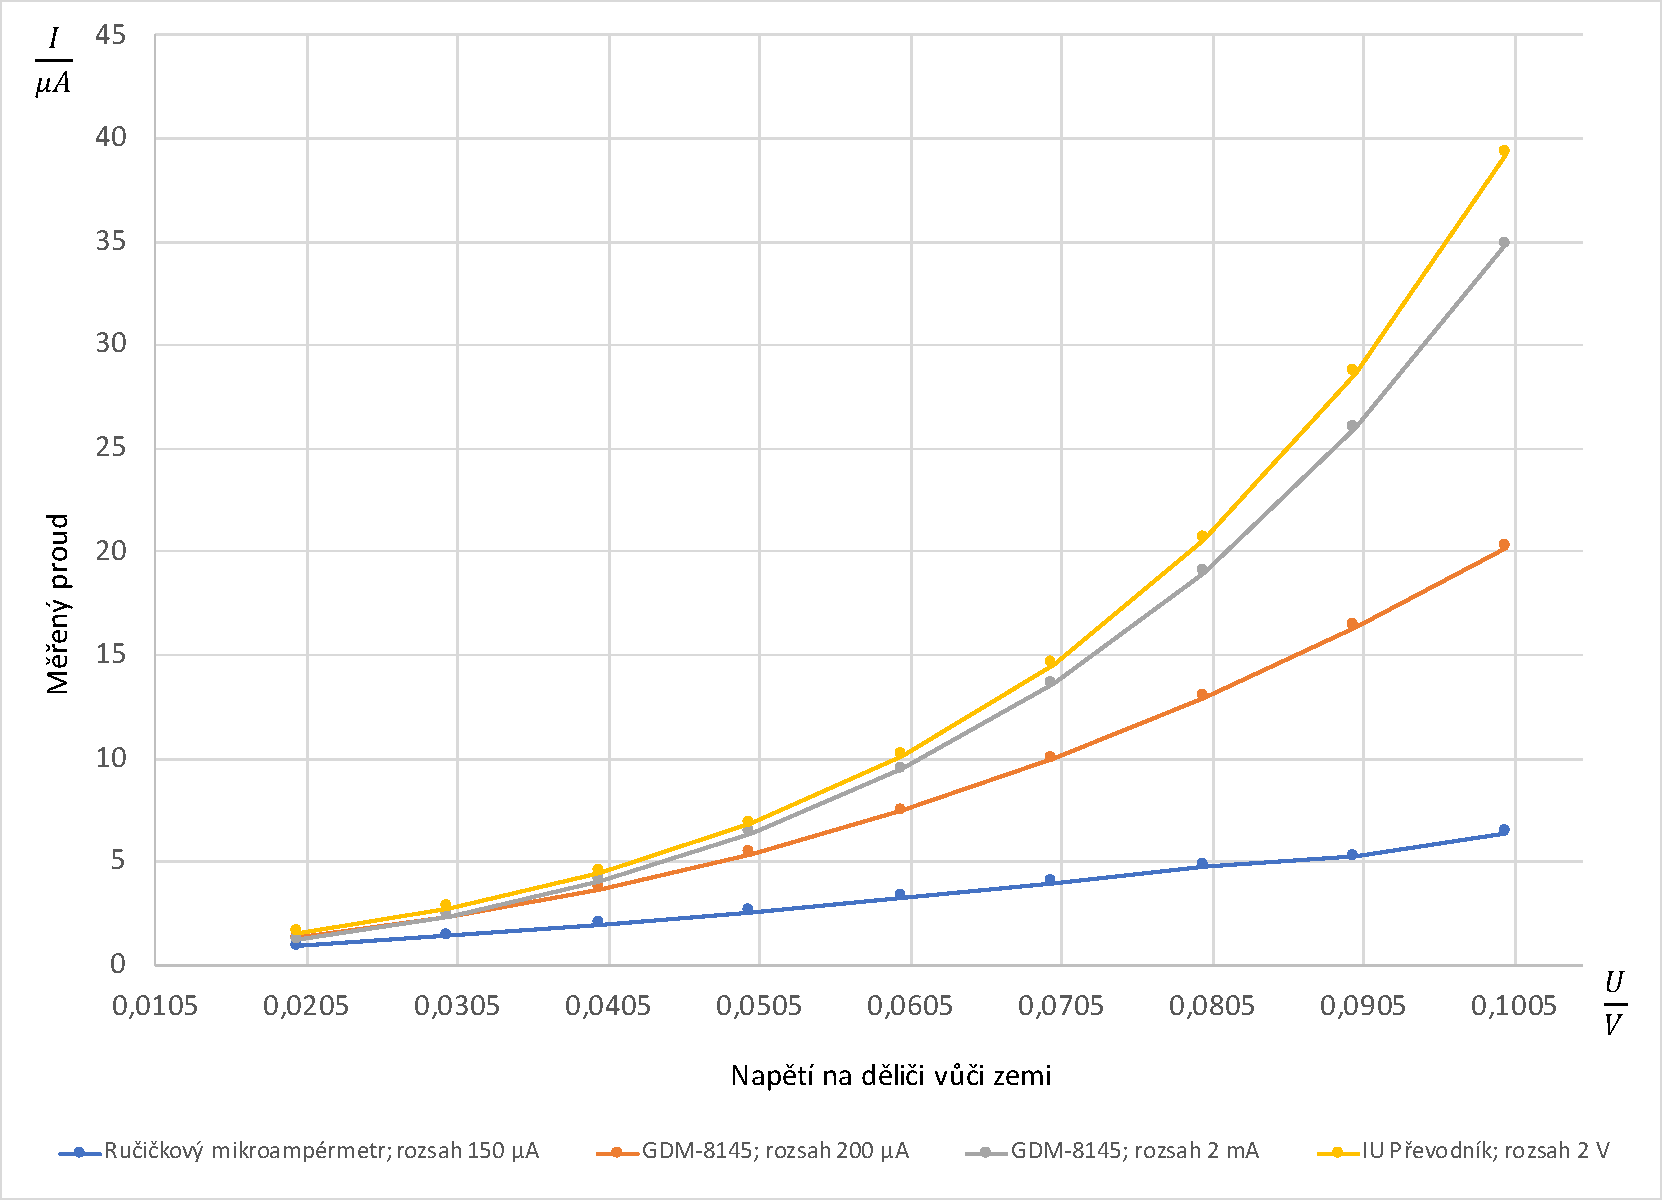
\includegraphics[width=.8\textwidth]{graf_namereno.pdf}
    \caption{Naměřené hodnoty přepočtené na \tmu A}
    \label{graf:hodnoty}
\end{graf}


\section{Zpracování naměřených hodnot}


\section{Závěrečné vyhodnocení}



%--- LITERATURA a~ZDROJE (povinne) ---
\clearpage
\renewcommand{\refname}{Seznam použité literatury a~zdrojů informací} 
%\section*{Seznam použité literatury a~zdrojů informací}
\phantomsection %pridej odkaz do PDF zalozek
\addcontentsline{toc}{section}{Seznam použité literatury a~zdrojů informací}

\begin{thebibliography}{99}

%----------------------------------------------------
\subsection*{Seznam použitých internetových zdrojů}
    \bibitem{navod} Návod k laboratorní úloze
    
\end{thebibliography}

\end{document}